\mysubsubsection{Black-Box Testen}

%%%%%%%%%%%%%%%%%%%%%%%%%%%%%%%%%

\begin{frame}
\frametitle{Black Box vs. White Box Testen}
  \begin{center}
  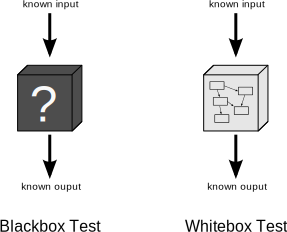
\includegraphics[width=.8\textwidth]{Qualitaetssicherung/abbildungen/BlackBoxAndWhiteBoxTesting}
  \end{center}
\end{frame}

%%%%%%%%%%%%%%%%%%%%%%%%%%%%%%%%%

\begin{frame}
\frametitle{Blackbox Testen von Modulen}
\begin{itemize}
  \item Idee: Ein Programmteil wird ohne Ansicht des Codes getestet.
  \item Problem: Wie bestimmt man dann die Testmenge? 
  \item Zur Bestimmung der Testmenge kann nur die Spezifikation herangezogen werden.
  \item Voraussetzung zur systematischen Generierung von Testmengen sind dann formale Spezifikationen.
\end{itemize}
\end{frame}

%%%%%%%%%%%%%%%%%%%%%%%%%%%%%%%%%

\begin{frame}
\frametitle{Mittelalterliches Beispiel}
L�sungen f�r Gleichungen der Form:
\begin{equation*}
  x^3 + ax^2 + bx + c = 0
\end{equation*}
 
\begin{itemize}
  \item 1535: Tartaglia hat eine L�sung gefunden, aber nicht verraten.
  \item Fior legte 30 Aufgaben zur �berpr�fung vor.
  \item Siehe: \citep{Wussing_Arnold1975}
\end{itemize}
\end{frame}

%%%%%%%%%%%%%%%%%%%%%%%%%%%%%%%%%

\begin{frame}
\frametitle{Mittelalterlicher Blackboxtext}
\setlength{\unitlength}{0.1\textwidth}
\begin{center}
\begin{picture}(9,5)
\put(0,5){\makebox(0,0)[tl]{Tartaglia}}
\put(9,5){\makebox(0,0)[tr]{Fior}}
\put(9,4){\makebox(0,0)[tr]{berechnet $(x-r)(x-s)(x-t)$}}
\put(4.5,3.3){\makebox(0,0){$x^3+ax^2+bx+c = 0$}}
\put(7,3){\vector(-1,0){5}}
\put(4.5,1.8){\makebox(0,0){r', s', t'}}
\put(2,1.5){\vector(1,0){5}}
\put(9,1){\makebox(0,0)[tr]{pr�ft $r=r', s=s', t=t'$}}
\end{picture}
\end{center}
\end{frame}


%%%%%%%%%%%%%%%%%%%%%%%%%%%%%%%%%
%
%\begin{frame}
%\frametitle{Blackbox Testen}
%\begin{center}
%\hspace*{4em} \pgfimage[width=0.8\textwidth]{Qualitaetssicherung/abbildungen/BlackboxTesten}
%\end{center}
%\end{frame}
%
%%%%%%%%%%%%%%%%%%%%%%%%%%%%%%%%%%
%
%\begin{frame}
%\frametitle{Beispiel: Testen eines Parsers}
%\underline{Idee:}
%\begin{center}
%\pgfimage[width=0.9\textwidth]{Qualitaetssicherung/abbildungen/Beispiel_Testen_eines_Parsers}
%\end{center}
%\end{frame}

%%%%%%%%%%%%%%%%%%%%%%%%%%%%%%%%%

\begin{frame}
\frametitle{Black Box Testverfahren}
\begin{itemize}
  \item Testf�lle aus der Programmspezifikation ableiten.
  \item Programmstruktur wird nicht betrachtet.
  \item M�glichst umfassende, aber redundanzarme Pr�fung der spezifizierten Funktionalit�t.
  \item Funktions�berdeckung ist das Ziel
  \item Testfallbestimmung: 
    \begin{itemize}
      \item Funktionale �quivalenzklassenbildung 
      \item Grenzwertanalyse 
      \item Test spezieller Werte
    \end{itemize}
\end{itemize}
\end{frame}

%%%%%%%%%%%%%%%%%%%%%%%%%%%%%%%%%

\begin{frame}
\frametitle{Funktionale �quivalenzklassenbildung}
\structure{Ziel}\\
Definitionsbereiche der Eingabeparameter und Wertebereiche der Ausgabeparameter werden in �quivalenzklassen zerlegt.
 
\vspace{\baselineskip}
\structure{Annahme}\\
Ein Programm reagiert bei der Verarbeitung eines Repr�sentanten aus einer �quivalenzklasse so, wie bei allen anderen Werten aus dieser �quivalenzklasse.
 
\vspace{\baselineskip}
\structure{Repr�sentant f�r einen Testfall}\\
Irgendein Element aus der Klasse ausw�hlen.
\end{frame}

%%%%%%%%%%%%%%%%%%%%%%%%%%%%%%%%%%

%\begin{frame}
%\frametitle{�quivalenzklassenbildung}
%\begin{center}
%\pgfimage[width=0.5\textwidth]{Qualitaetssicherung/abbildungen/Aequivalenzklassenbildung}
%\end{center}
%\end{frame}

%%%%%%%%%%%%%%%%%%%%%%%%%%%%%%%%%

\begin{frame}
\frametitle{Grenzwertanalyse}
\begin{itemize}
  \item Testf�lle, die die Grenzwerte der �quivalenzklassen abdecken oder in der unmittelbaren Umgebung dieser Grenzen liegen, decken besonders h�ufig Fehler auf.
  \item Es wird nicht irgendein Element aus der �quivalenzklasse als Repr�sentant ausgew�hlt.
  \item Es werden ein oder mehrere Elemente ausgesucht, so dass jeder Rand der �quivalenzklasse getestet wird.
\end{itemize}
\end{frame}

%%%%%%%%%%%%%%%%%%%%%%%%%%%%%%%%%

\begin{frame}
\frametitle{�quivalenzklassen mit Grenzwerten}
\begin{center}
\pgfimage[width=0.95\textwidth]{Qualitaetssicherung/abbildungen/AequivalenzklassenMitGrenzwerten}
\end{center}
\end{frame}

%%%%%%%%%%%%%%%%%%%%%%%%%%%%%%%%%

\begin{frame}
\frametitle{Spezifikation einer Suchfunktion}
\begin{tabbing}
\hspace*{2em} \= \hspace{2em} \= \kill
\textbf{procedure} Search (Key : ELEM ; T: ELEM\_ARRAY;\\
\> Found : \textbf{in out} BOOLEAN; L: \textbf{in out} ELEM\_INDEX) ;\\[1 em]
\textbf{Pre-condition}\\
\> \> -- the array has at least one element\\
\> \> T'FIRST <= T'LAST\\
\textbf{Post-condition}\\
\> \> -- the element is found and is referenced by L\\
\> \> ( Found and T (L) = Key) \\
\> \> \textbf{or}\\
\> \> -- the element is not in the array\\
\> \> ( \textbf{not} Found \textbf{and} \\
\> \> \textbf{not} (\textbf{exists} i, T'FIRST >= i <= T'LAST, T (i) = Key ))
\end{tabbing}
\end{frame}

%%%%%%%%%%%%%%%%%%%%%%%%%%%%%%%%%

\begin{frame}
\frametitle{�quivalenzklassenbildung}
\framesubtitle{auf Basis der Spezifikation}
\begin{itemize}
  \item Eingaben, die die Vorbedingung erf�llen 
  \item Eingaben, die die Vorbedingung nicht erf�llen 
  \item Eingaben, bei denen das Schl�sselelement im Array ist 
  \item Eingaben, bei denen das Schl�sselelement nicht im Array ist 
  \item Eingabemengen
    \begin{itemize}
      \item Mit 0 Elementen 
      \item Mit 1 Element
      \item Mit mehreren Elementen
    \end{itemize}
\end{itemize}
\end{frame}

%%%%%%%%%%%%%%%%%%%%%%%%%%%%%%%%%

\begin{frame}
\frametitle{�quivalenzklassen f�r die Suchfunktion}
\begin{tabular}{l@{\hspace{2em}}l}\hline
\textbf{Array}      & \textbf{Element} \\ \hline 
Single value        & In sequence  \\ \hline   
Single value        & Not in sequence \\ \hline
More than 1 value   & First element in sequence \\ \hline
More than 1 value   & Last element in sequence  \\ \hline
More than 1 value   & Middle element in sequence \\ \hline
More than 1 value   & Not in sequence \\ \hline
\end{tabular}

\vspace{1em}
\begin{tabular}{l@{\hspace{2ex}}c@{\hspace{2ex}}l} \hline
\textbf{Input sequence} (T)  & \textbf{Key}  & \textbf{Output} (Found, L) \\ \hline
17                          & 17            & true, 1 \\ \hline
17                          & 0             & false, * \\ \hline
17, 29, 21, 23              & 17            & true, 1 \\ \hline
41, 18, 9, 31, 30, 16, 45   & 45            & true, 7 \\ \hline
17, 18, 21, 23, 29, 41, 38  & 23            & true, 4 \\ \hline
21, 23, 29, 33, 38          & 25            & false, * \\ \hline
\end{tabular}
\end{frame}

%%%%%%%%%%%%%%%%%%%%%%%%%%%%%%%%%

\begin{frame}
\frametitle{Black Box und White Box Testen}
  \begin{center}
  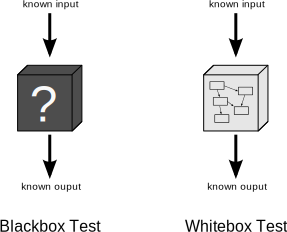
\includegraphics[width=.8\textwidth]{Qualitaetssicherung/abbildungen/BlackBoxAndWhiteBoxTesting}
  \end{center}
\end{frame}

%%%%%%%%%%%%%%%%%%%%%%%%%%%%%%%%%

\begin{frame}
\frametitle{Fuzzy Testing}
Fuzzing:
\begin{itemize}
	\item Anders als bei Unit-Tests werden beim Fuzzy-Testing Testf�lle nicht manuell definiert, sondern anhand statistischer Funktionen zuf�llig erzeugt.
	\item Durch eine hohe Anzahl der so generierten Tests wird die Software auch auf au�ergew�hnliche Eingabeparameter getestet.
\begin{itemize}
	\item Das ist insbesondere zur Aufdeckung von Sicherheitsl�cken interessant.
\end{itemize}
\item Fuzzing wird in der Regel im Rahmen eines Black-Box-Tests durchgef�hrt, um neue Software auf Fehleranf�lligkeit zu pr�fen sowie um Sicherheitsl�cken aufzusp�ren.
\item Wenn das Programm bei bestimmten vom Fuzzer generierten Daten reproduzierbar ein Problem verursacht (z. B.\ abst�rzt), kann darauf aufbauend anhand von White-Box-Tests die genaue Ursache gesucht werden. 
\end{itemize}
\end{frame}

%%%%%%%%%%%%%%%%%%%%%%%%%%%%%%%%%

\begin{frame}
\frametitle{Test-Orakel}
  \begin{center}
  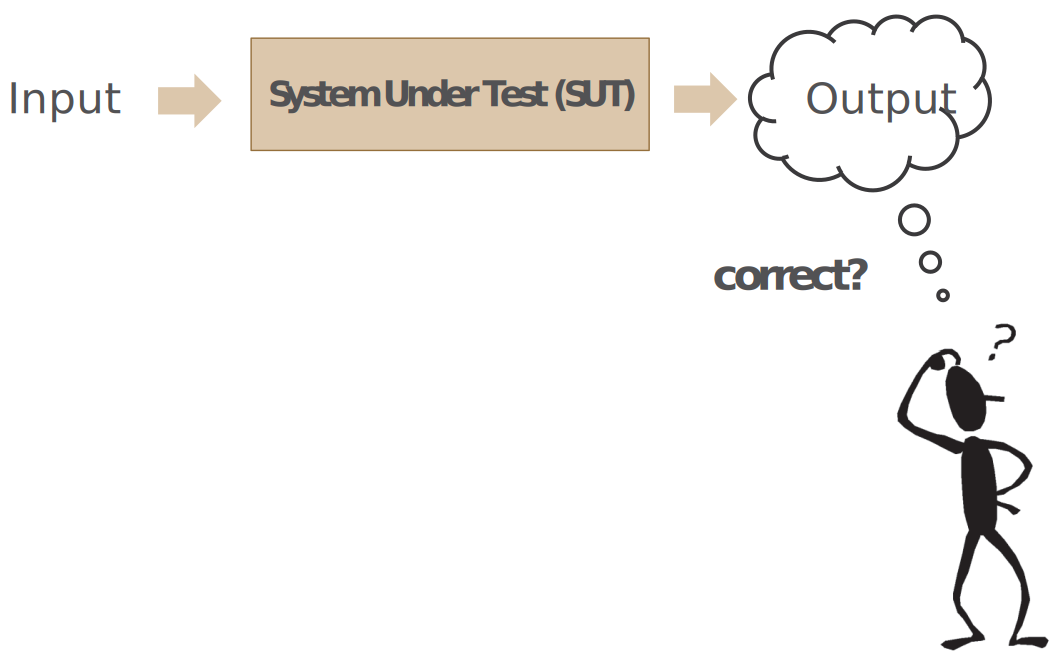
\includegraphics[width=\textwidth]{Qualitaetssicherung/abbildungen/TestOracle}
  \end{center}
\end{frame}

%%%%%%%%%%%%%%%%%%%%%%%%%%%%%%%%%

\begin{frame}
\frametitle{F�r welche Art von Software gibt es keine Test-Orakel?}
  \begin{center}
  \url{https://monti.com}
  \end{center}
\end{frame}

%%%%%%%%%%%%%%%%%%%%%%%%%%%%%%%%%

\begin{frame}
\frametitle{Das Orakel-Problem}
\framesubtitle{Es ist nicht immer m�glich, ein Orakel zu definieren}
  \begin{center}
\only<beamer>{\includegraphics[width=\textwidth]{Qualitaetssicherung/abbildungen/TestOracleProblem}}
  \end{center}
	Was tun? \\
	\citet{MetamorphicTesting2016,segura_metamorphic_2020,kanewala_metamorphic_2019}
\end{frame}

%%%%%%%%%%%%%%%%%%%%%%%%%%%%%%%%%

\begin{frame}
\frametitle{Anwendungsbereiche f�r metamorphisches Testen}
\framesubtitle{\citet{segura_metamorphic_2020}}
  \begin{center}
\only<beamer>{\includegraphics[width=.65\textwidth]{Qualitaetssicherung/abbildungen/MetamorphicTesting}}
  \end{center}
\end{frame}

